\chapter{Appendix A}
\section{Upper-Air Charts}
Images provided by the NOAA/ESRL Physical Science Division, Boulder, Colorado. Original data can be found at \url{http://www.esrl.noaa.gov/psd/}.
\begin{figure}
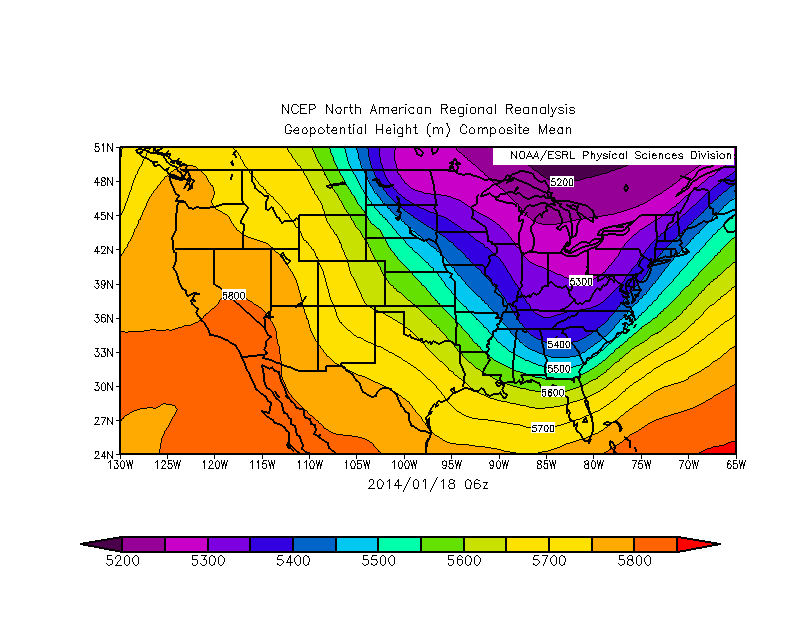
\includegraphics[width=\textwidth, trim={2cm 1.5cm 2cm 3cm},clip]{500mb/20140118_06Z_GPH}
\caption{500mb Geopotential Height at 06Z 18 January 2014.} 
\label{fig:gph_20140118}
\end{figure}


\begin{figure}
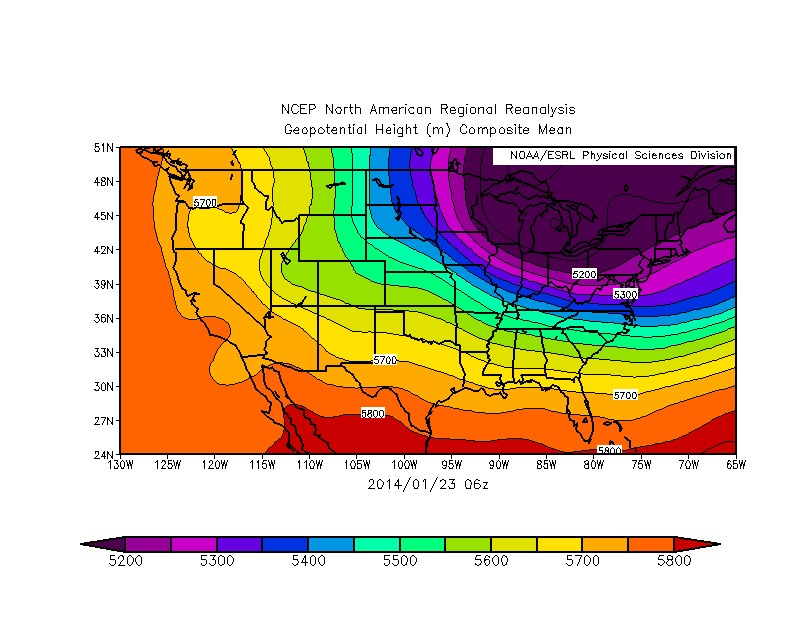
\includegraphics[width=\textwidth, trim={2cm 1.5cm 2cm 3cm},clip]{500mb/20140123_06Z_GPH}
\caption{500mb Geopotential Height at 06Z 23 January 2014} 
\label{fig:gph_20140123}
\end{figure}

\begin{figure}
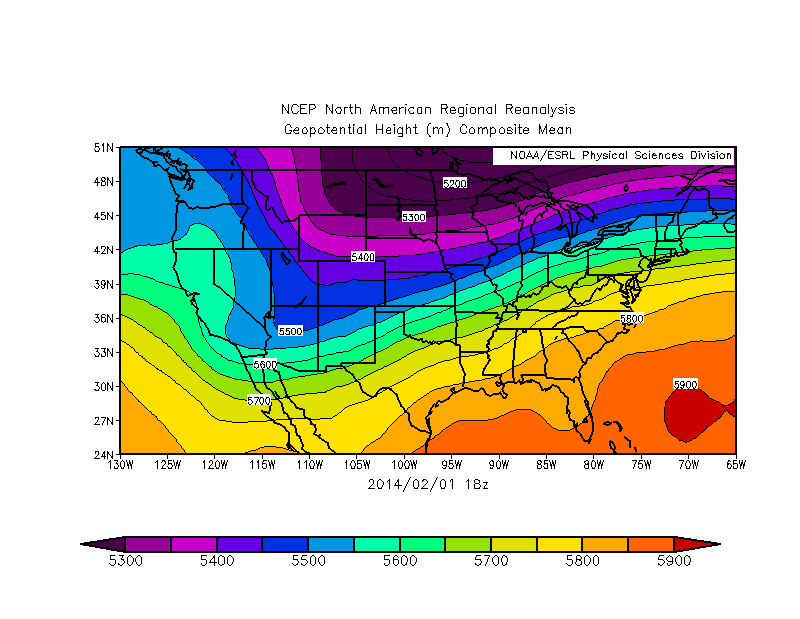
\includegraphics[width=\textwidth, trim={2cm 1.5cm 2cm 3cm},clip]{500mb/20140201_18Z_GPH}
\caption{500mb Geopotential Height at 18Z 1 February 2014.}
\label{fig:gph_20140106}
\end{figure}

\begin{figure}
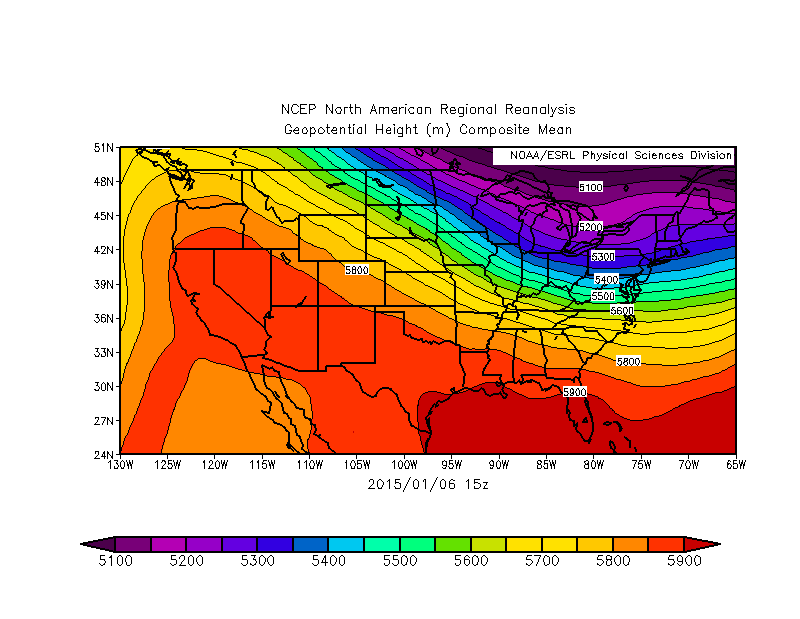
\includegraphics[width=\textwidth, trim={2cm 1.5cm 2cm 3cm},clip]{500mb/20150106_15Z_GPH}
\caption{500mb Geopotential Height at 15Z 6 January 2015.} 
\label{fig:gph_20150106}
\end{figure}


\begin{figure}
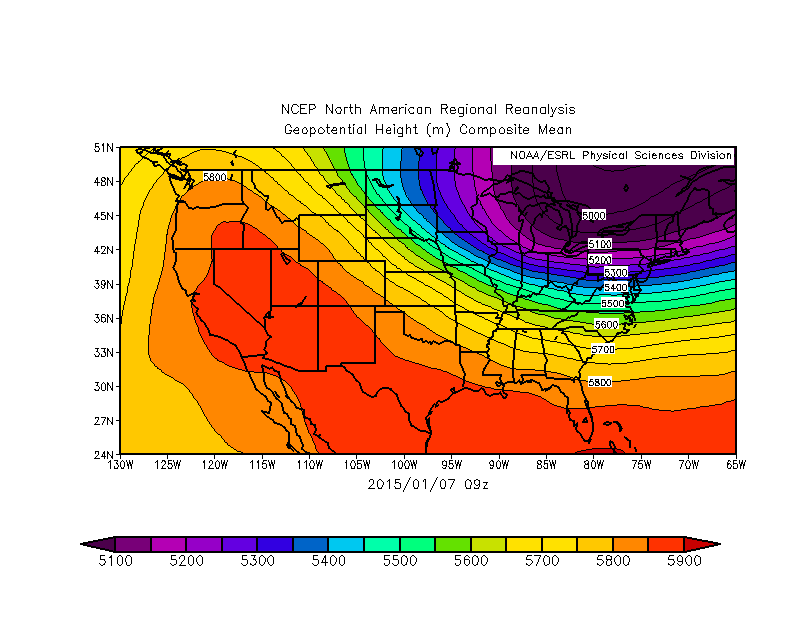
\includegraphics[width=\textwidth, trim={2cm 1.5cm 2cm 3cm},clip]{500mb/20150107_09Z_GPH}
\caption{500mb Geopotential Height at 09Z 7 January 2015.} 
\label{fig:gph_20150107}
\end{figure}


\begin{figure}
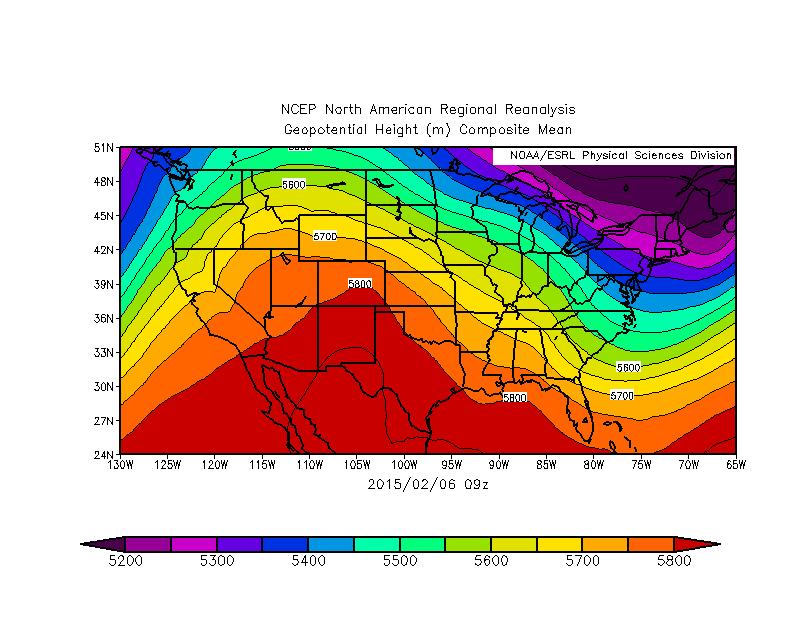
\includegraphics[width=\textwidth, trim={2cm 1.5cm 2cm 3cm},clip]{500mb/20150206_09Z_GPH}
\caption{500mb Geopotential Height at 09Z 6 February 2015.} 
\label{fig:gph_20150206}
\end{figure}


\begin{figure}
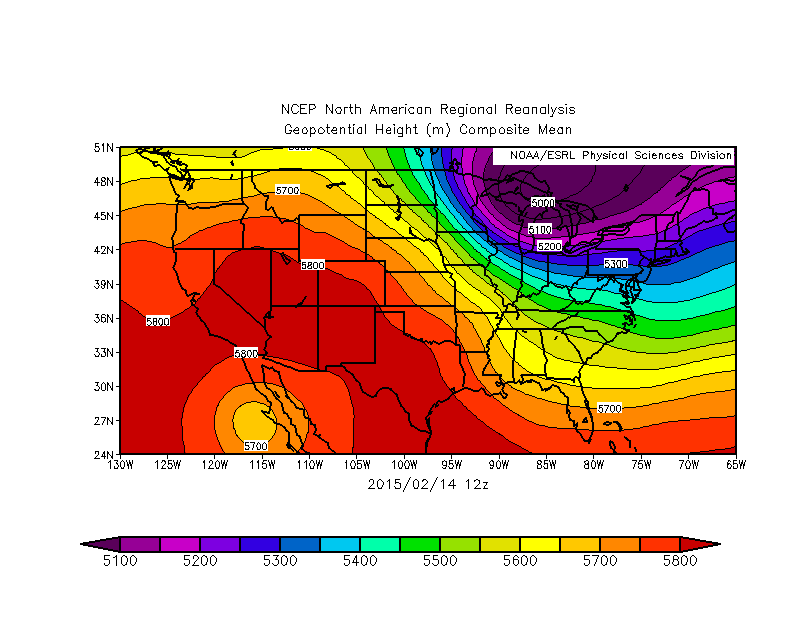
\includegraphics[width=\textwidth, trim={2cm 1.5cm 2cm 3cm},clip]{500mb/20150214_12Z_GPH}
\caption{500mb Geopotential Height at 12Z 14 February 2015.} 
\label{fig:gph_20150214}
\end{figure}


\begin{figure}
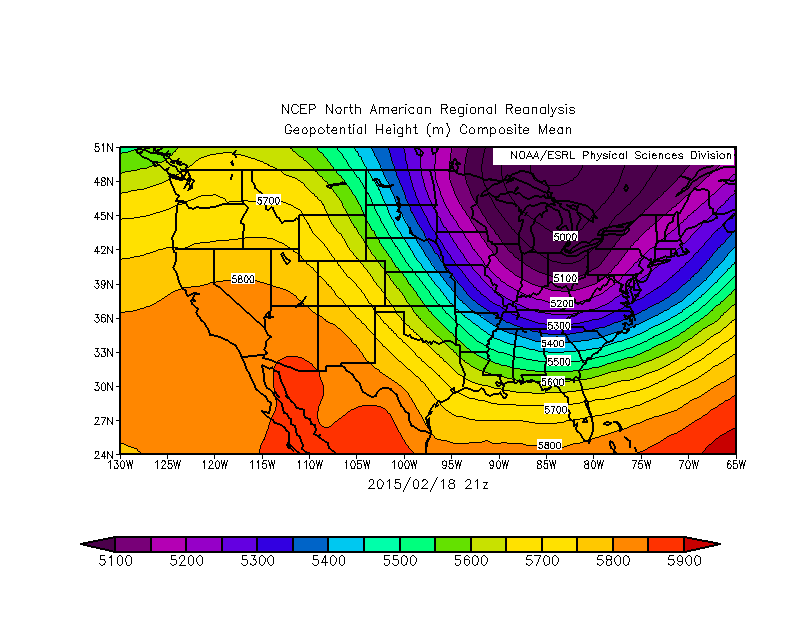
\includegraphics[width=\textwidth, trim={2cm 1.5cm 2cm 3cm},clip]{500mb/20150218_21Z_GPH}
\caption{500mb Geopotential Height at 21Z 18 February 2015.} 
\label{fig:gph_20150218}
\end{figure}


\begin{figure}
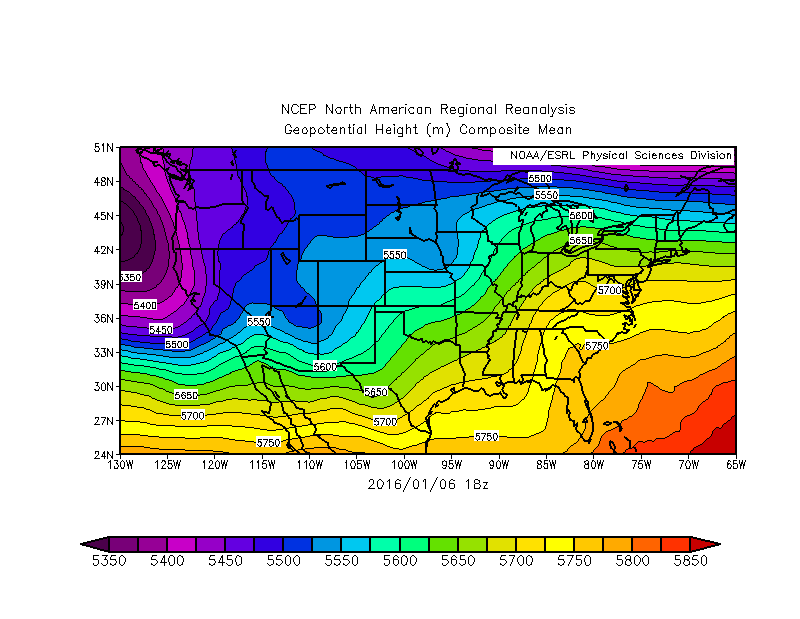
\includegraphics[width=\textwidth, trim={2cm 1.5cm 2cm 3cm},clip]{500mb/20160210_18Z_GPH}
\caption{500mb Geopotential Height at 18Z 10 February 2016.} 
\label{fig:gph_20160210}
\end{figure}


\begin{figure}
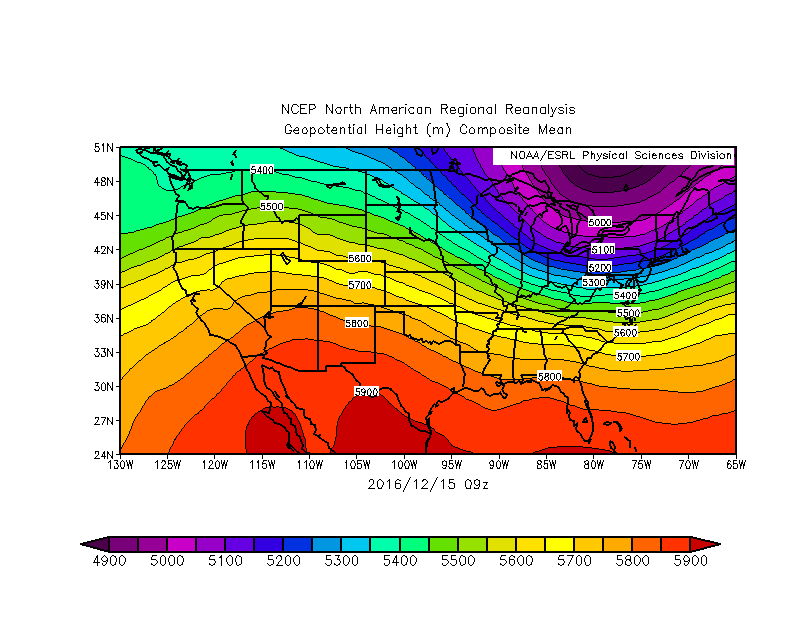
\includegraphics[width=\textwidth, trim={2cm 1.5cm 2cm 3cm},clip]{500mb/20161215_09Z_GPH}
\caption{500mb Geopotential Height at 09Z 15 December 2016.} 
\label{fig:gph_20161215}
\end{figure}

\section{Skew-T Charts}
Raw sounding data provided by the Department of Atmospheric Science at the University of Wyoming. Original data can be found at \url{http://weather.uwyo.edu/upperair/sounding.html}.
\begin{figure}
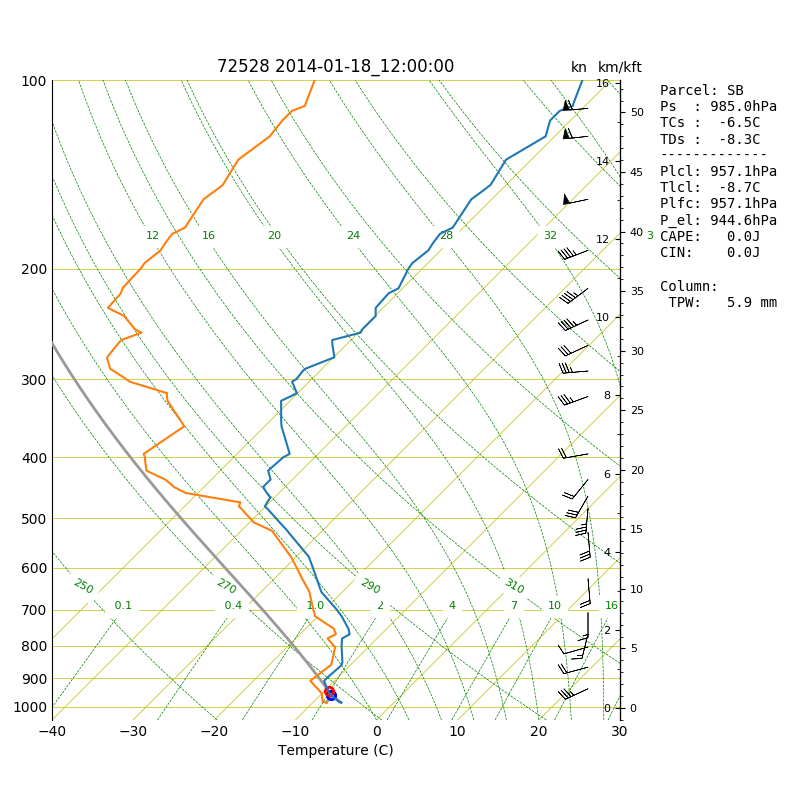
\includegraphics[width=\textwidth]{skewt/sounding_20140118_12Z}
\caption{SkewT/Log-P Chart from the BUF Radiosonde launched at 12Z 18 January 2014} 
\label{fig:skewt_20140123}
\end{figure}

\begin{figure}
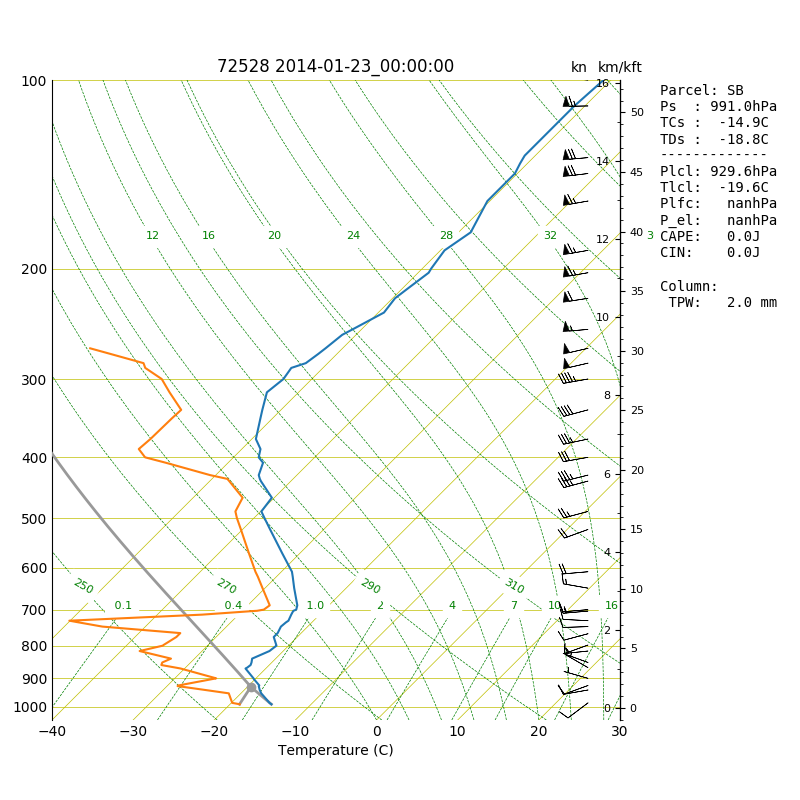
\includegraphics[width=\textwidth]{skewt/sounding_20140123_00Z}
\caption{SkewT/Log-P Chart from the BUF Radiosonde launched at 00Z 23 January 2014} 
\label{fig:skewt_20140123}
\end{figure}

\begin{figure}
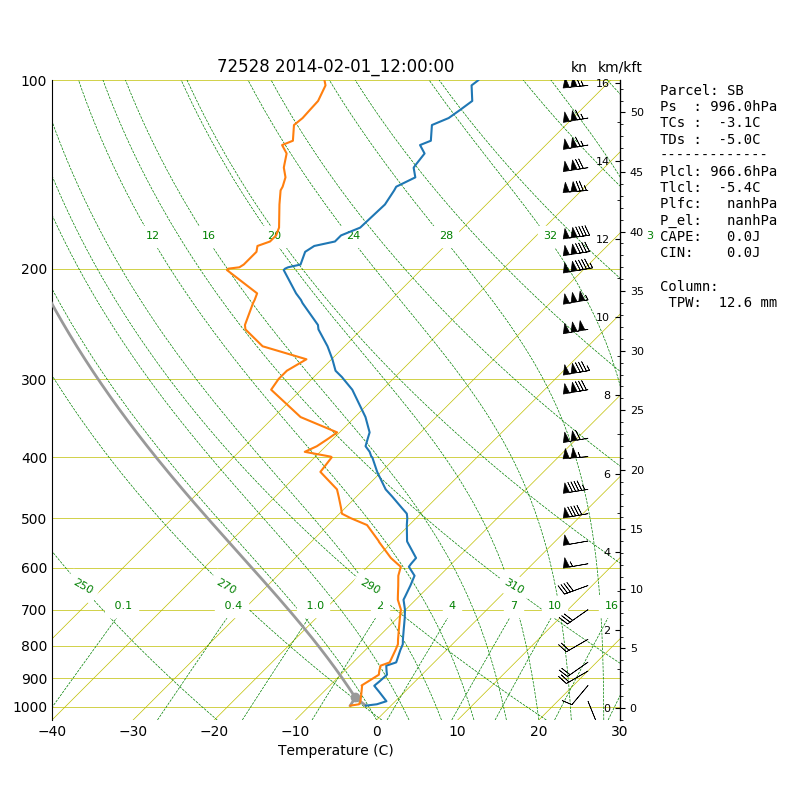
\includegraphics[width=\textwidth]{skewt/sounding_20140201_12Z}
\caption{SkewT/Log-P Chart from the BUF Radiosonde launched at 12Z 1 February 2014} 
\label{fig:skewt_20140201}
\end{figure}

\begin{figure}
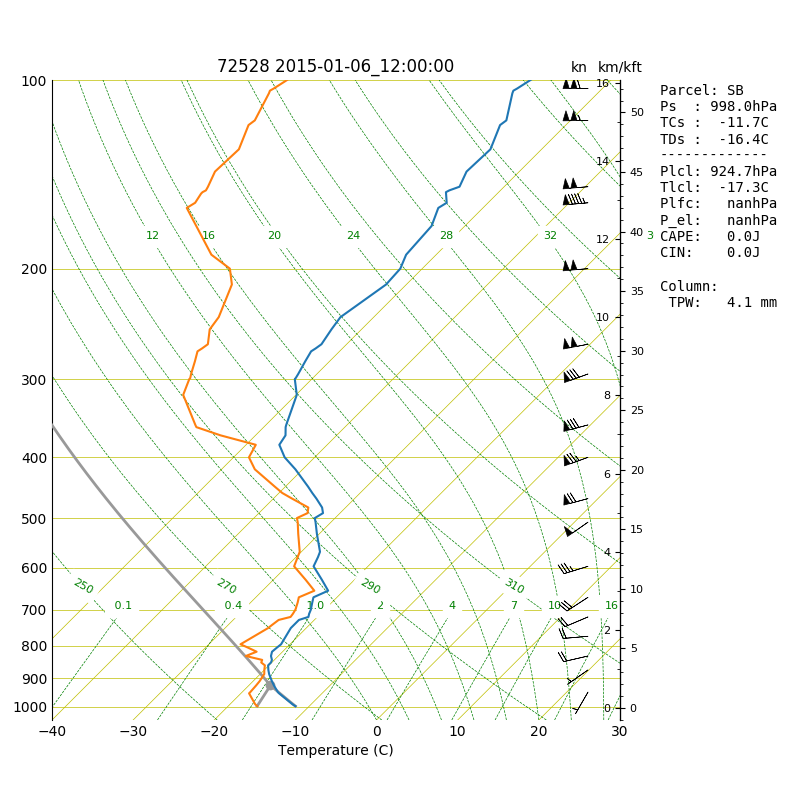
\includegraphics[width=\textwidth]{skewt/sounding_20150106_12Z}
\caption{SkewT/Log-P Chart from the BUF Radiosonde launched at 00Z 6 January 2015} 
\label{fig:skewt_20150106}
\end{figure}

\begin{figure}
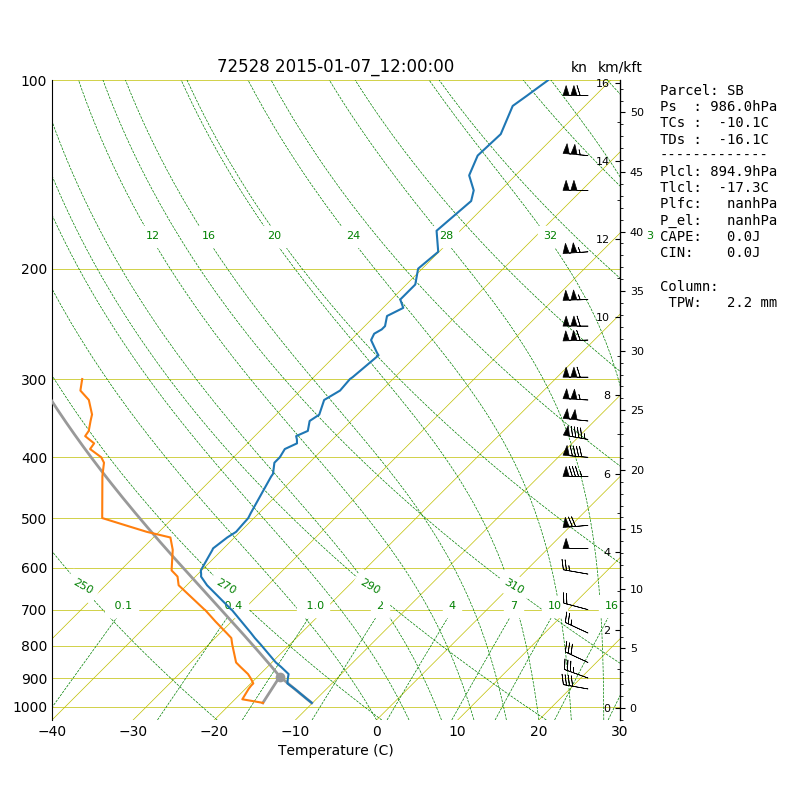
\includegraphics[width=\textwidth]{skewt/sounding_20150107_12Z}
\caption{SkewT/Log-P Chart from the BUF Radiosonde launched at 12Z 7 January 2015} 
\label{fig:skewt_20150107}
\end{figure}

\begin{figure}
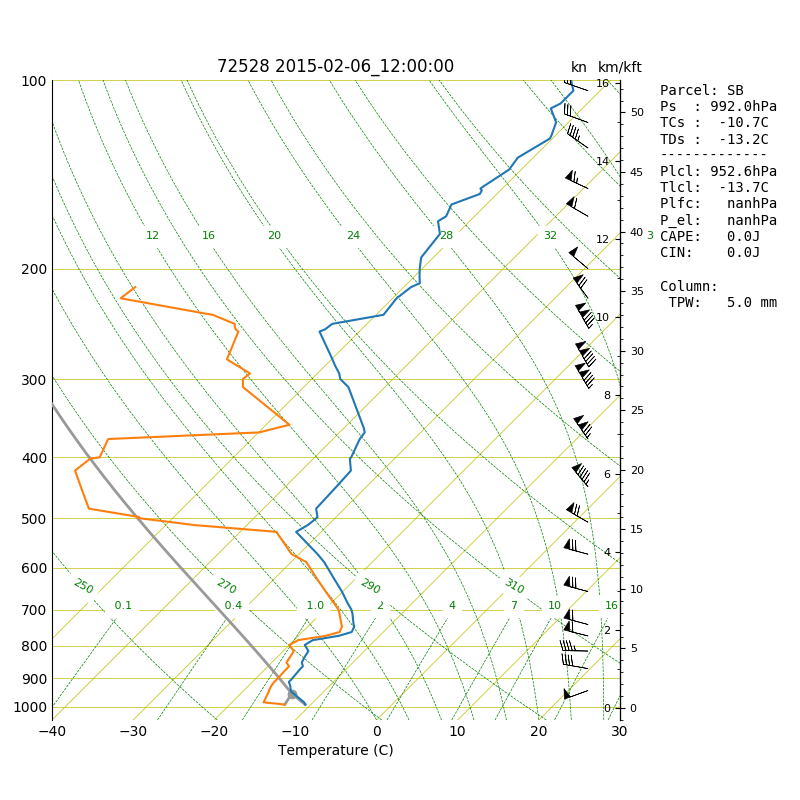
\includegraphics[width=\textwidth]{skewt/sounding_20150206_12Z}
\caption{SkewT/Log-P Chart from the BUF Radiosonde launched at 00Z 6 February 2015} 
\label{fig:skewt_20150206}
\end{figure}

\begin{figure}
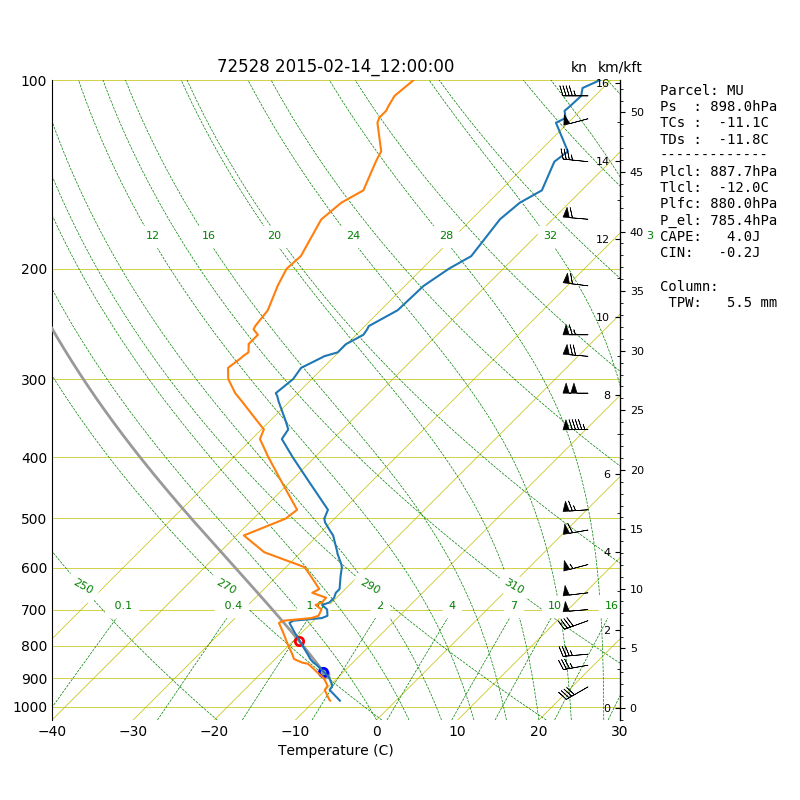
\includegraphics[width=\textwidth]{skewt/sounding_20150214_12Z}
\caption{SkewT/Log-P Chart from the BUF Radiosonde launched at 12Z 14 February 2015} 
\label{fig:skewt_20150214}
\end{figure}

\begin{figure}
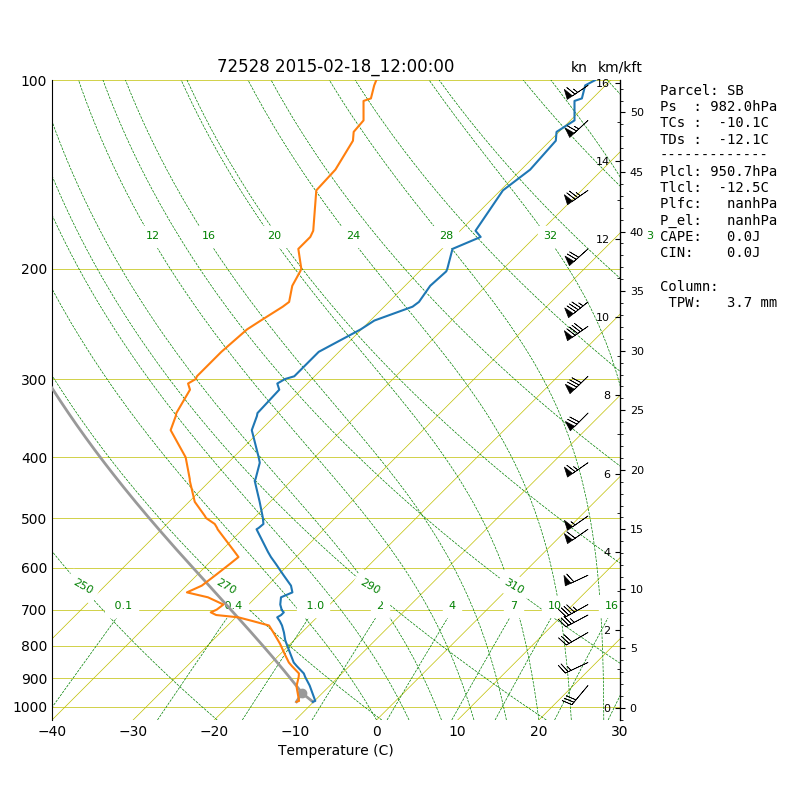
\includegraphics[width=\textwidth]{skewt/sounding_20150218_12Z}
\caption{SkewT/Log-P Chart from the BUF Radiosonde launched at 00Z 18 February 2015} 
\label{fig:skewt_20150218}
\end{figure}

\begin{figure}
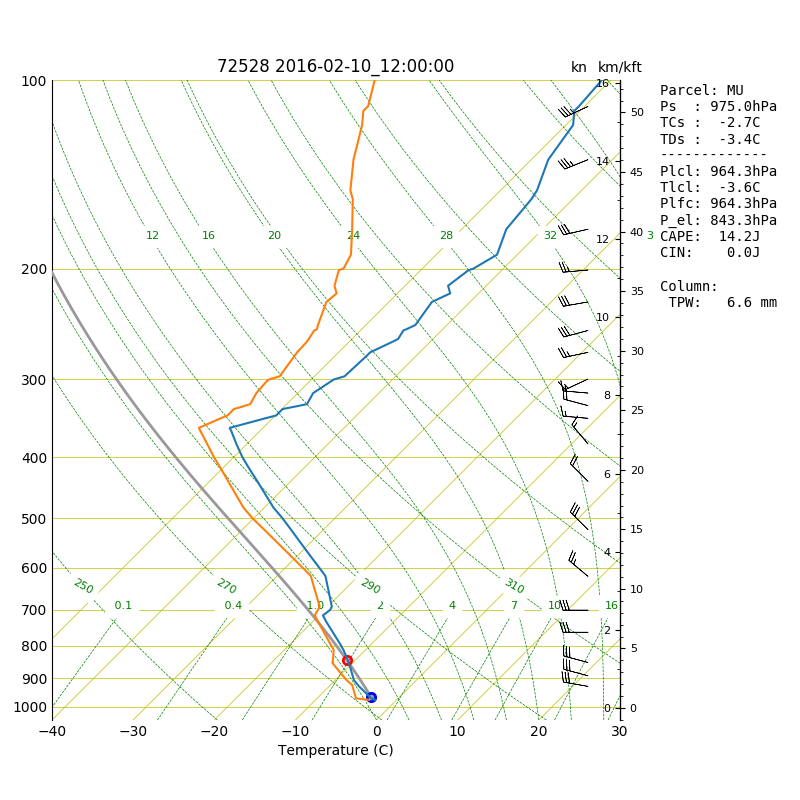
\includegraphics[width=\textwidth]{skewt/sounding_20160210_12Z}
\caption{SkewT/Log-P Chart from the BUF Radiosonde launched at 12Z 10 February 2016} 
\label{fig:skewt_20160210}
\end{figure}

\begin{figure}
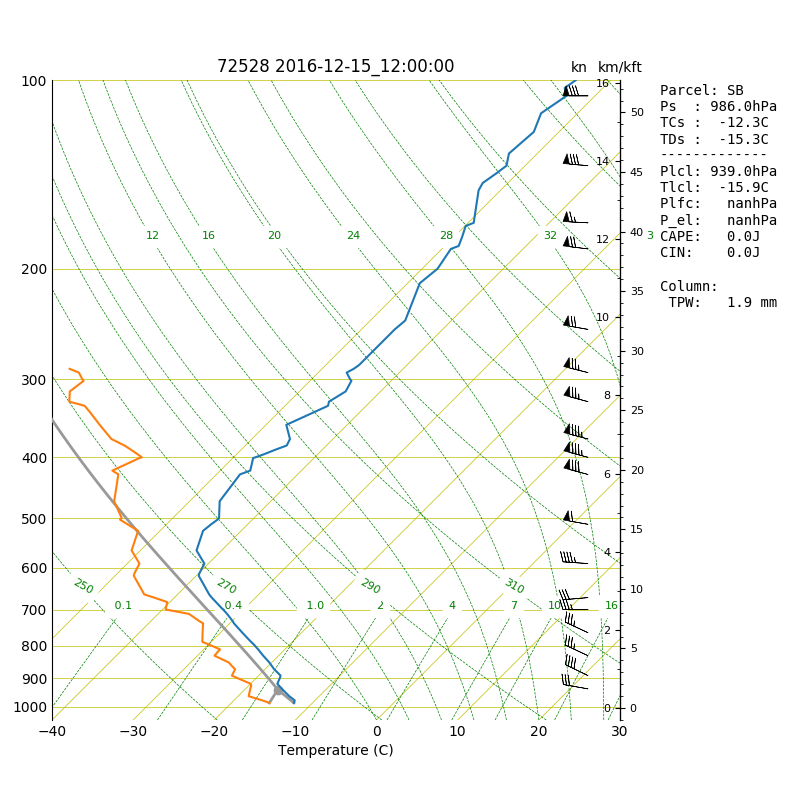
\includegraphics[width=\textwidth]{skewt/sounding_20161215_12Z}
\caption{SkewT/Log-P Chart from the BUF Radiosonde launched at 12Z 15 December 2016} 
\label{fig:skewt_20161215}
\end{figure}

\section{Sounding Climatology}
Images provided by the National Weather Service Storm Prediction Center in Norman, Oklahoma. Original data can be found at \url{http://www.spc.noaa.gov/exper/soundingclimo/}.
\begin{figure}
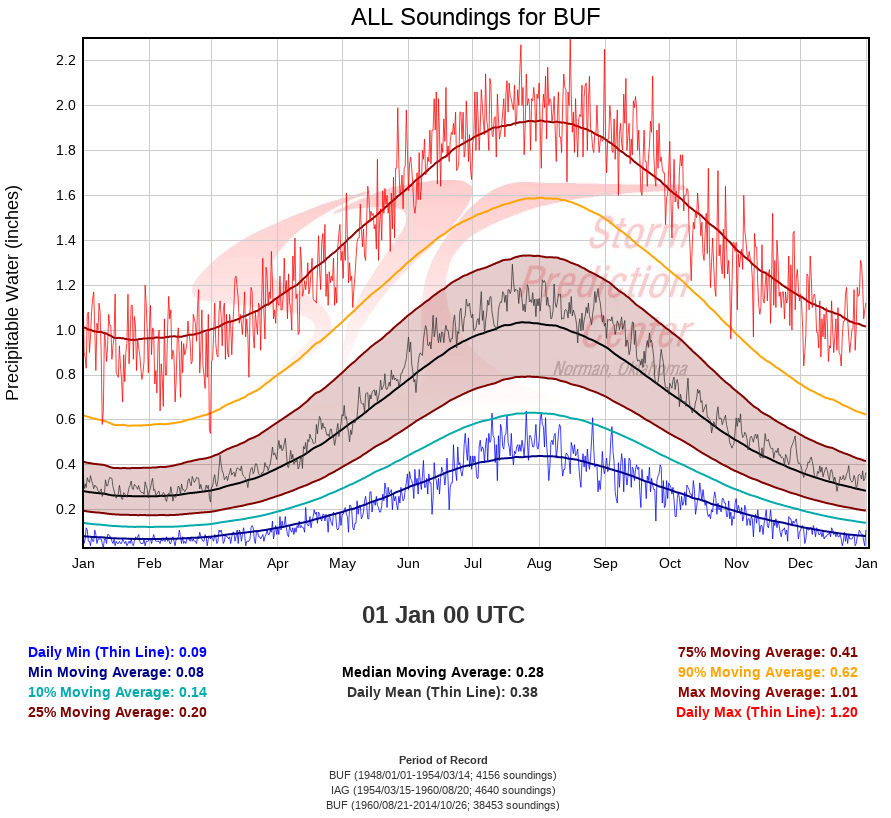
\includegraphics[width=\textwidth]{sounding_climo}
\caption{Sounding Precipitable Water Climatology for BUF} 
\label{fig:skewt_20161215}
\end{figure}